% !Mode:: "TeX:UTF-8"
% !TEX program  = xelatex
\documentclass[a4paper]{article}
\usepackage{amsmath}
\usepackage{amssymb}
\usepackage[UTF8]{ctex}
\usepackage{graphicx}
\usepackage[european]{circuitikz}
\usepackage{multirow}
\usepackage{geometry}
\usepackage{listings}
\usepackage{float}
% wkl's C/C++ and python latex settings
\lstset{
	language=[ANSI]{C},
	numbers=left,
	numberstyle=\color[RGB]{0,192,192},
	backgroundcolor=\color[RGB]{245,245,244},
	basicstyle=\ttfamily\small,
	breakatwhitespace=false,
	breaklines=true,
	captionpos=b,
	commentstyle=\color{gray},
	directivestyle=\color{blue},
	extendedchars=false,
	framexleftmargin=8mm,
	framexrightmargin=8mm,
	framerule=0pt,
	keywordstyle=\color{blue}\bfseries,
	morekeywords={*,define,*,include...},
	numbersep=5pt,
	rulesepcolor=\color{red!20!green!20!blue!20},
	showspaces=false,
	showstringspaces=false,
	showtabs=false,
	stringstyle=\color{purple},
	tabsize=4,
	title=\lstname
	}

\geometry{a4paper, top=2.54cm, bottom=2.54cm, left=3.18cm, right=3.18cm}
\title{电子电路电路实验 \\ 智能元件参数测试仪报告}
\author{王凯灵 521030910356 \\ 张杭磊 521030910358 \\ 代铭波 519030910364}
\date{2022年12月12日}
\begin{document}
	\maketitle
	\section{原选题工作}
	本组原来选择了超声波的题目。此前已经完成了超声波发生电路。电路采用MAX232芯片，基本电路如图\ref{mx232}所示。
	\begin{figure}[h]
	    \centering
	    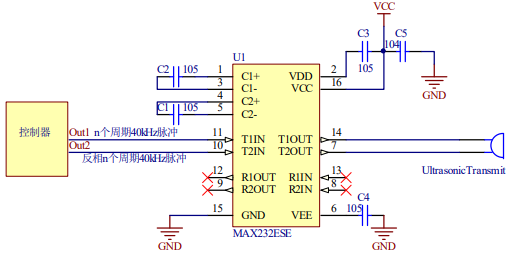
\includegraphics[width=0.5\linewidth]{图片/max232}
	    \caption{超声波发生电路图}
	    \label{mx232}
	\end{figure}
	
	其中，五个电容均使用了0.1$\mu F$。输入信号使用了40kHz的方波信号，vpp设置为3.5V（即芯片最低标准输入电压）。芯片和电路在面包板上的连线实物图如图\ref{mx232r}所示，近距离共地示波器波形如\ref{mx232s}所示，可以看出示波器钩子接收到了比较平整的同频率超声波方波信号。
	
	\begin{figure}[h]
	    \centering
	    \begin{minipage}[t]{0.49\linewidth}
	        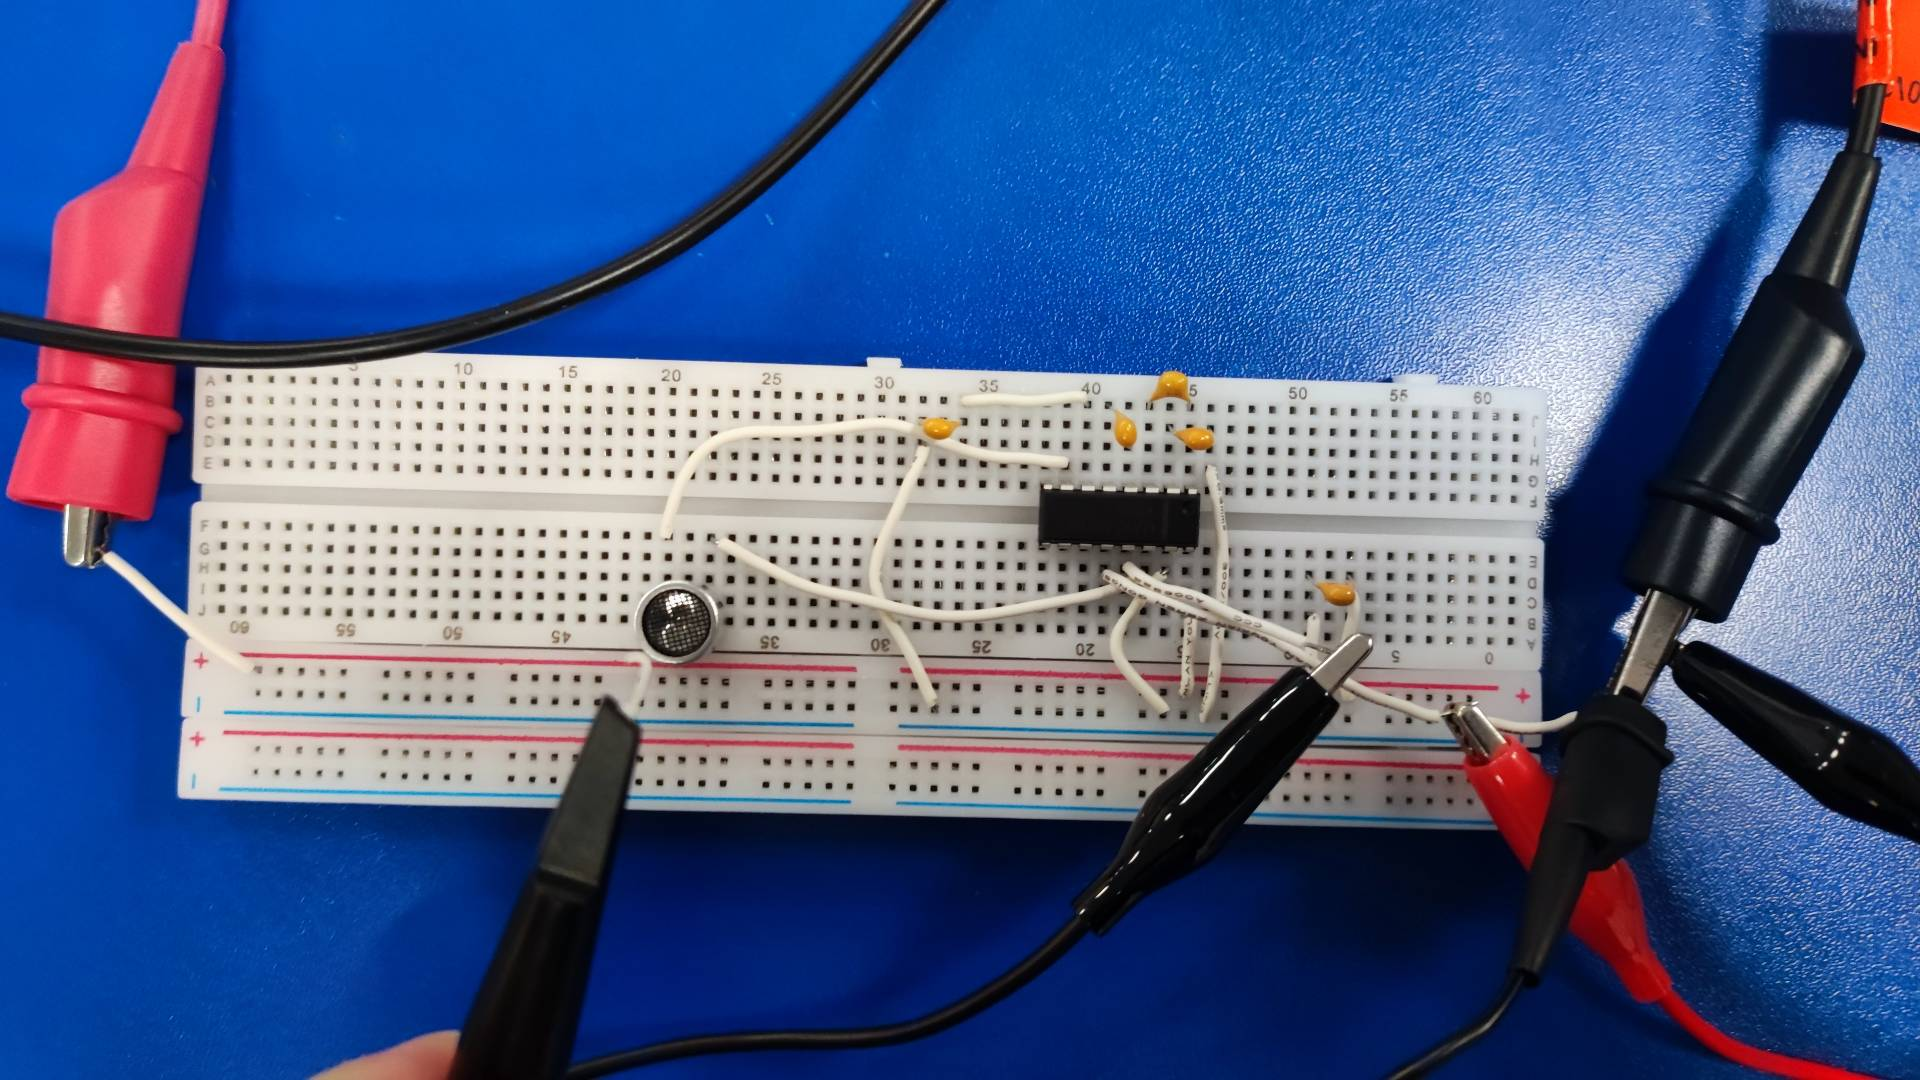
\includegraphics[width=1\linewidth]{图片/超声实物}
	        \caption{超声波发生电路实物图}
	        \label{mx232r}
	    \end{minipage}
	    \begin{minipage}[t]{0.49\linewidth}
	        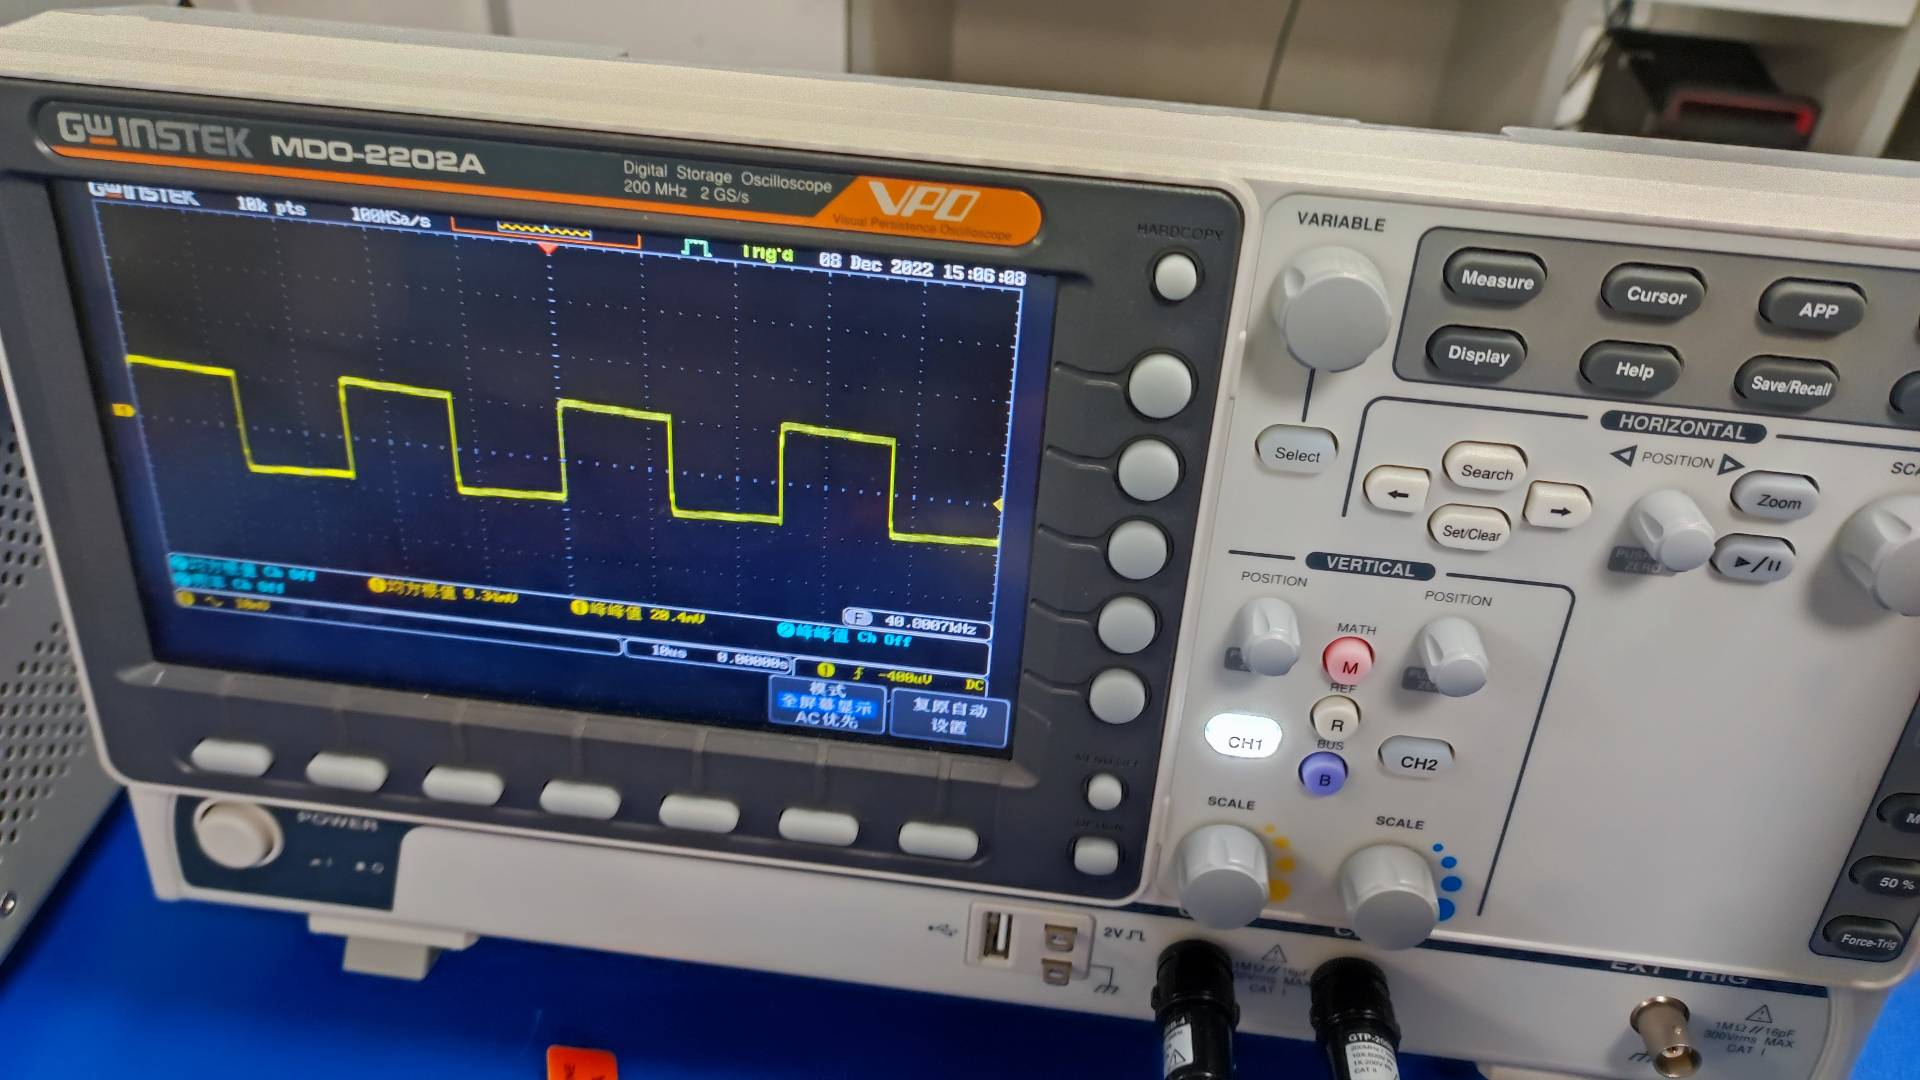
\includegraphics[width=1\linewidth]{图片/超声示波}
	        \caption{超声波示波器图像}
	        \label{mx232s}
	    \end{minipage}
	\end{figure}
	
	调整示波器接收端与发生器的距离。接收到的信号强弱随距离明显变化，首先于人类右臂长度，最远距离达到约一米，仍可以观察到信号。
	
	\begin{figure}[h]
	    \centering
	    \begin{minipage}[t]{0.32\linewidth}
	        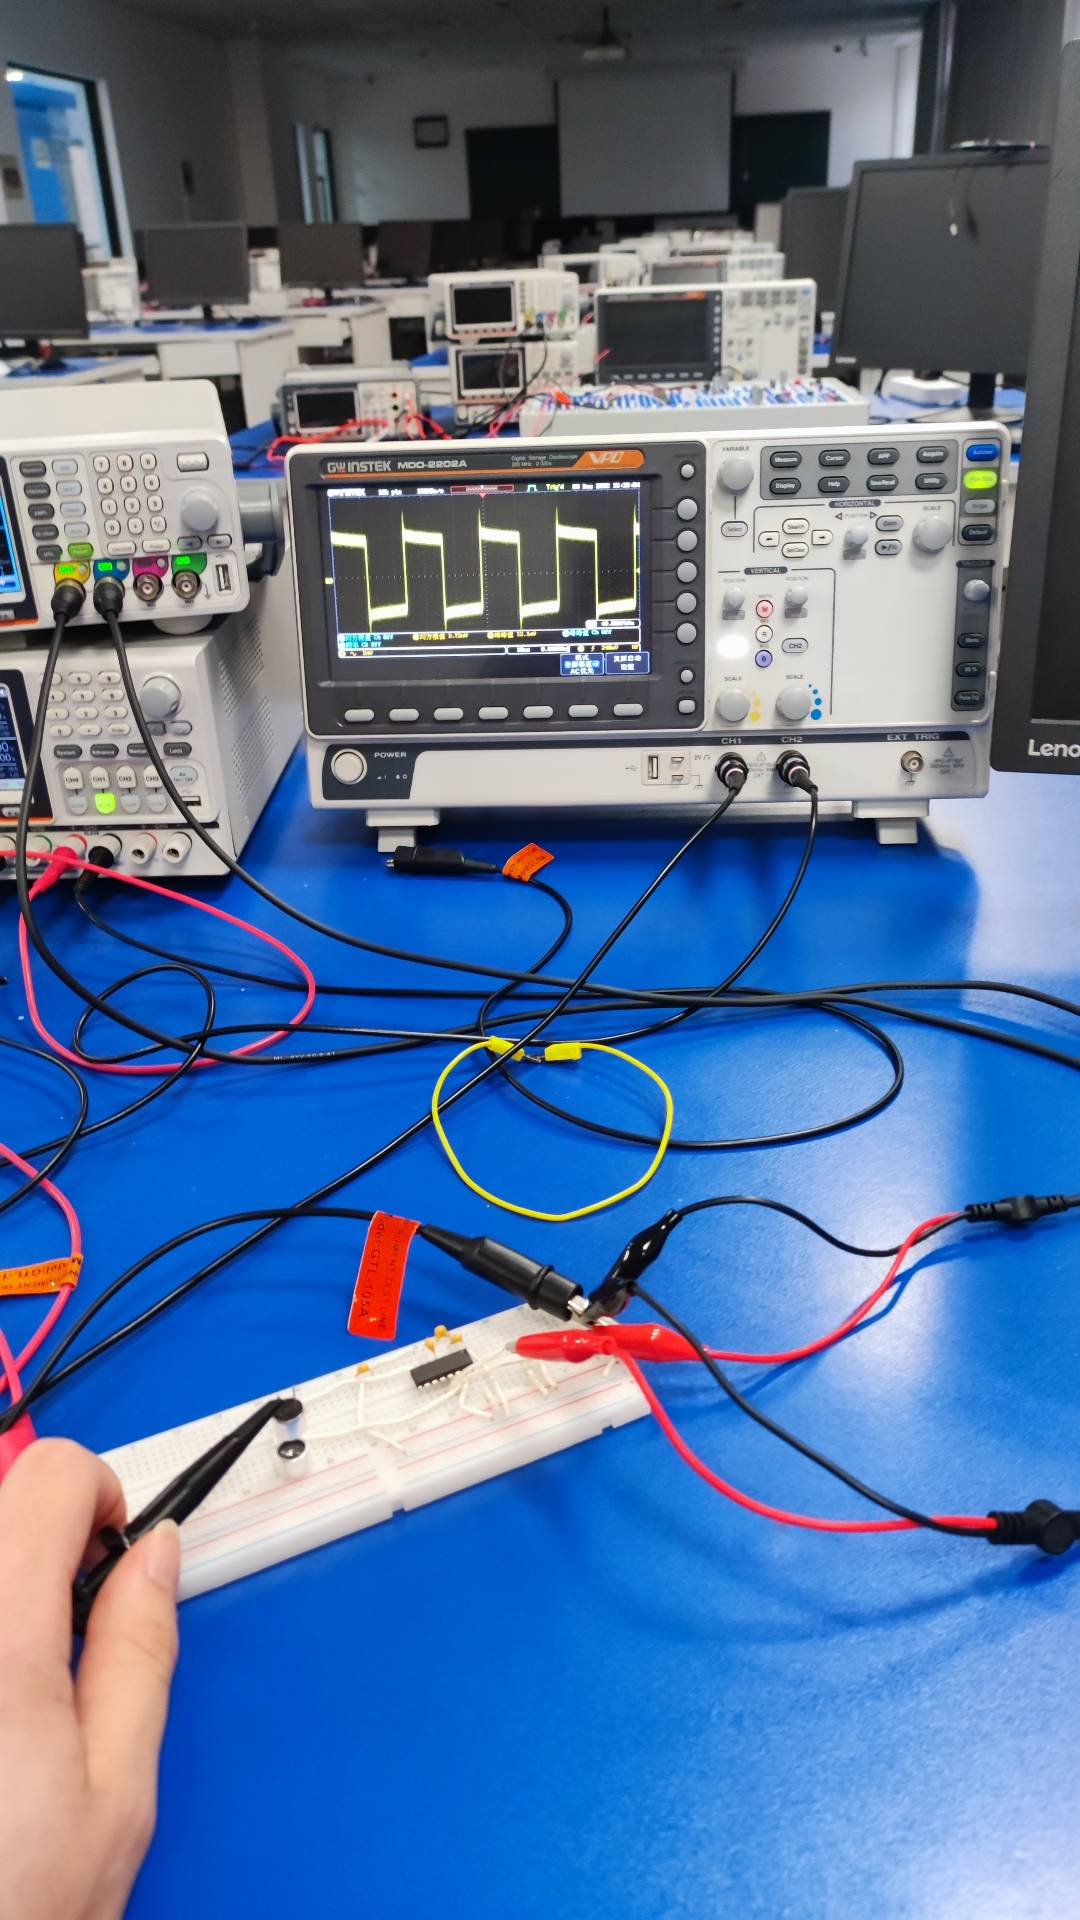
\includegraphics[width=0.9\linewidth]{图片/近距离}
	        \caption{近距离}
	        \label{mx232r}
	    \end{minipage}
	    \begin{minipage}[t]{0.32\linewidth}
	        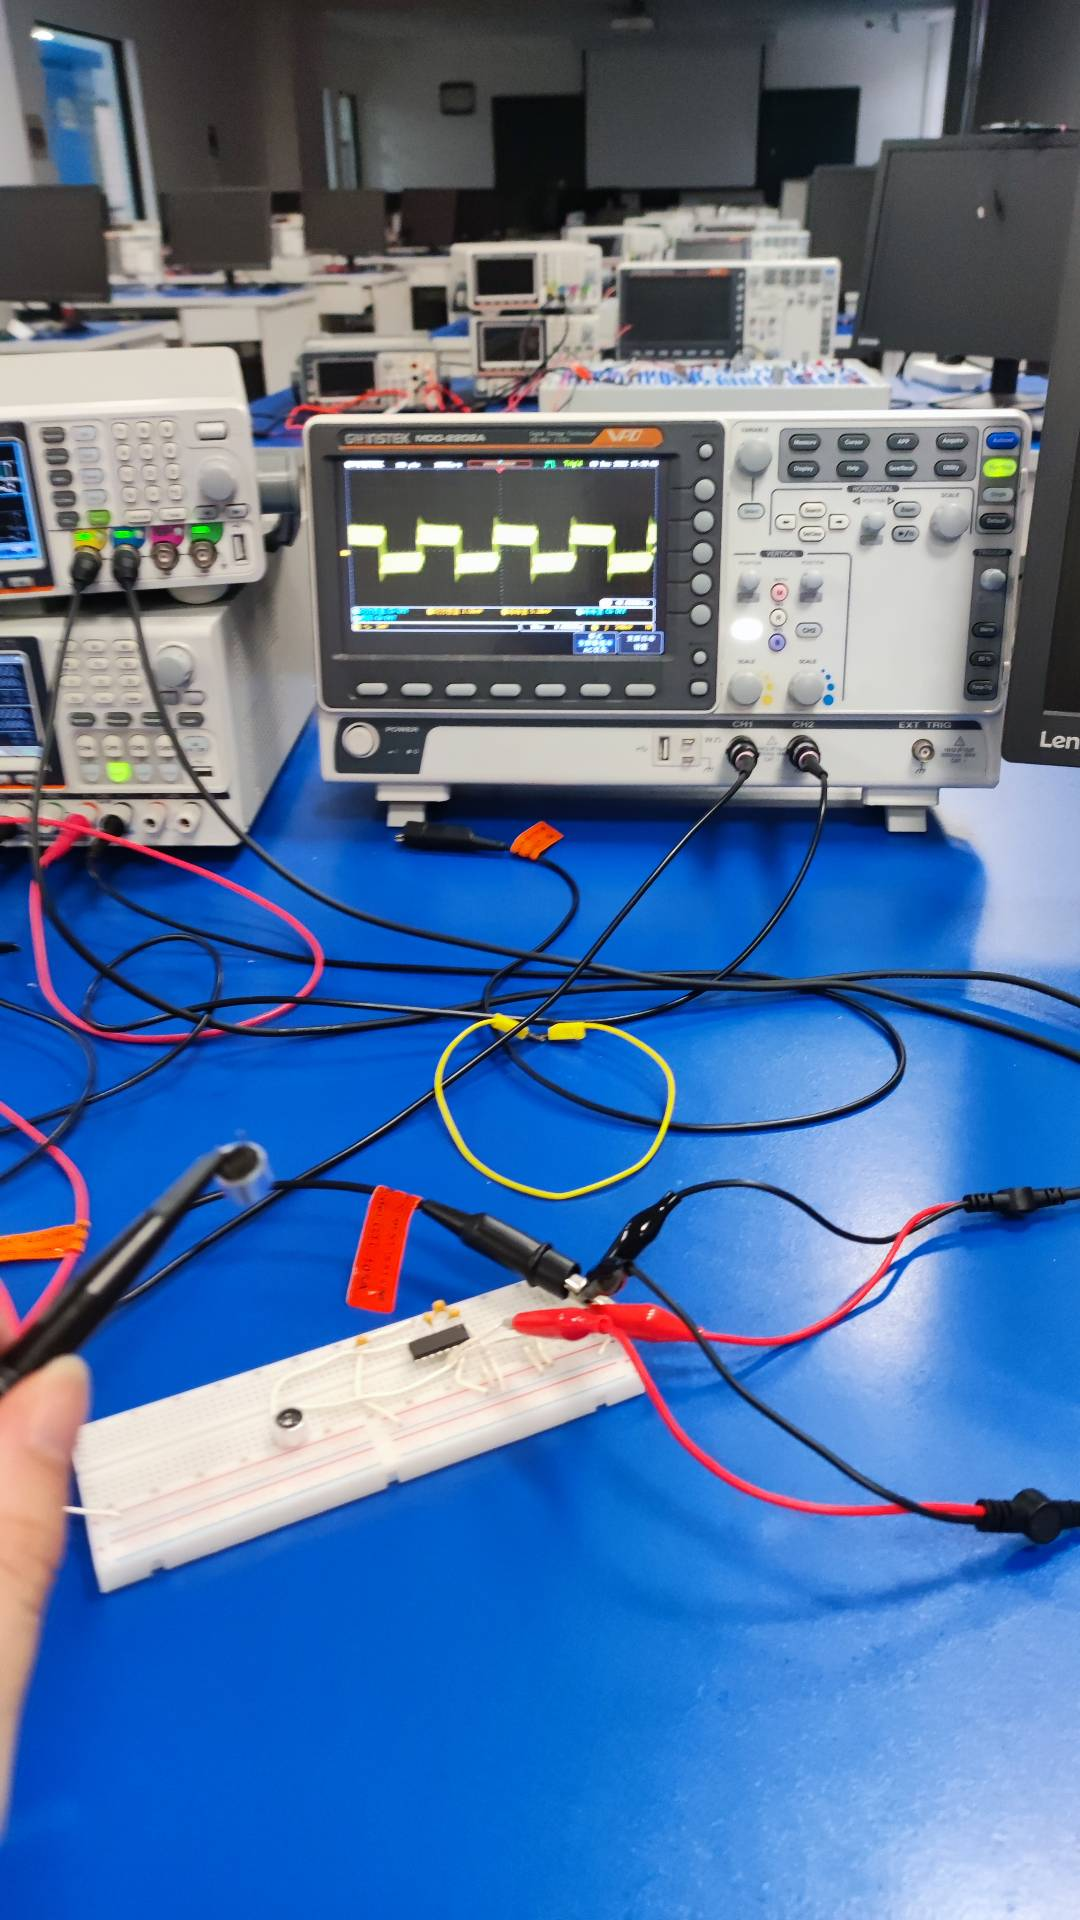
\includegraphics[width=0.9\linewidth]{图片/中距离}
	        \caption{中距离}
	        \label{mx232s}
	    \end{minipage}
        \begin{minipage}[t]{0.32\linewidth}
	        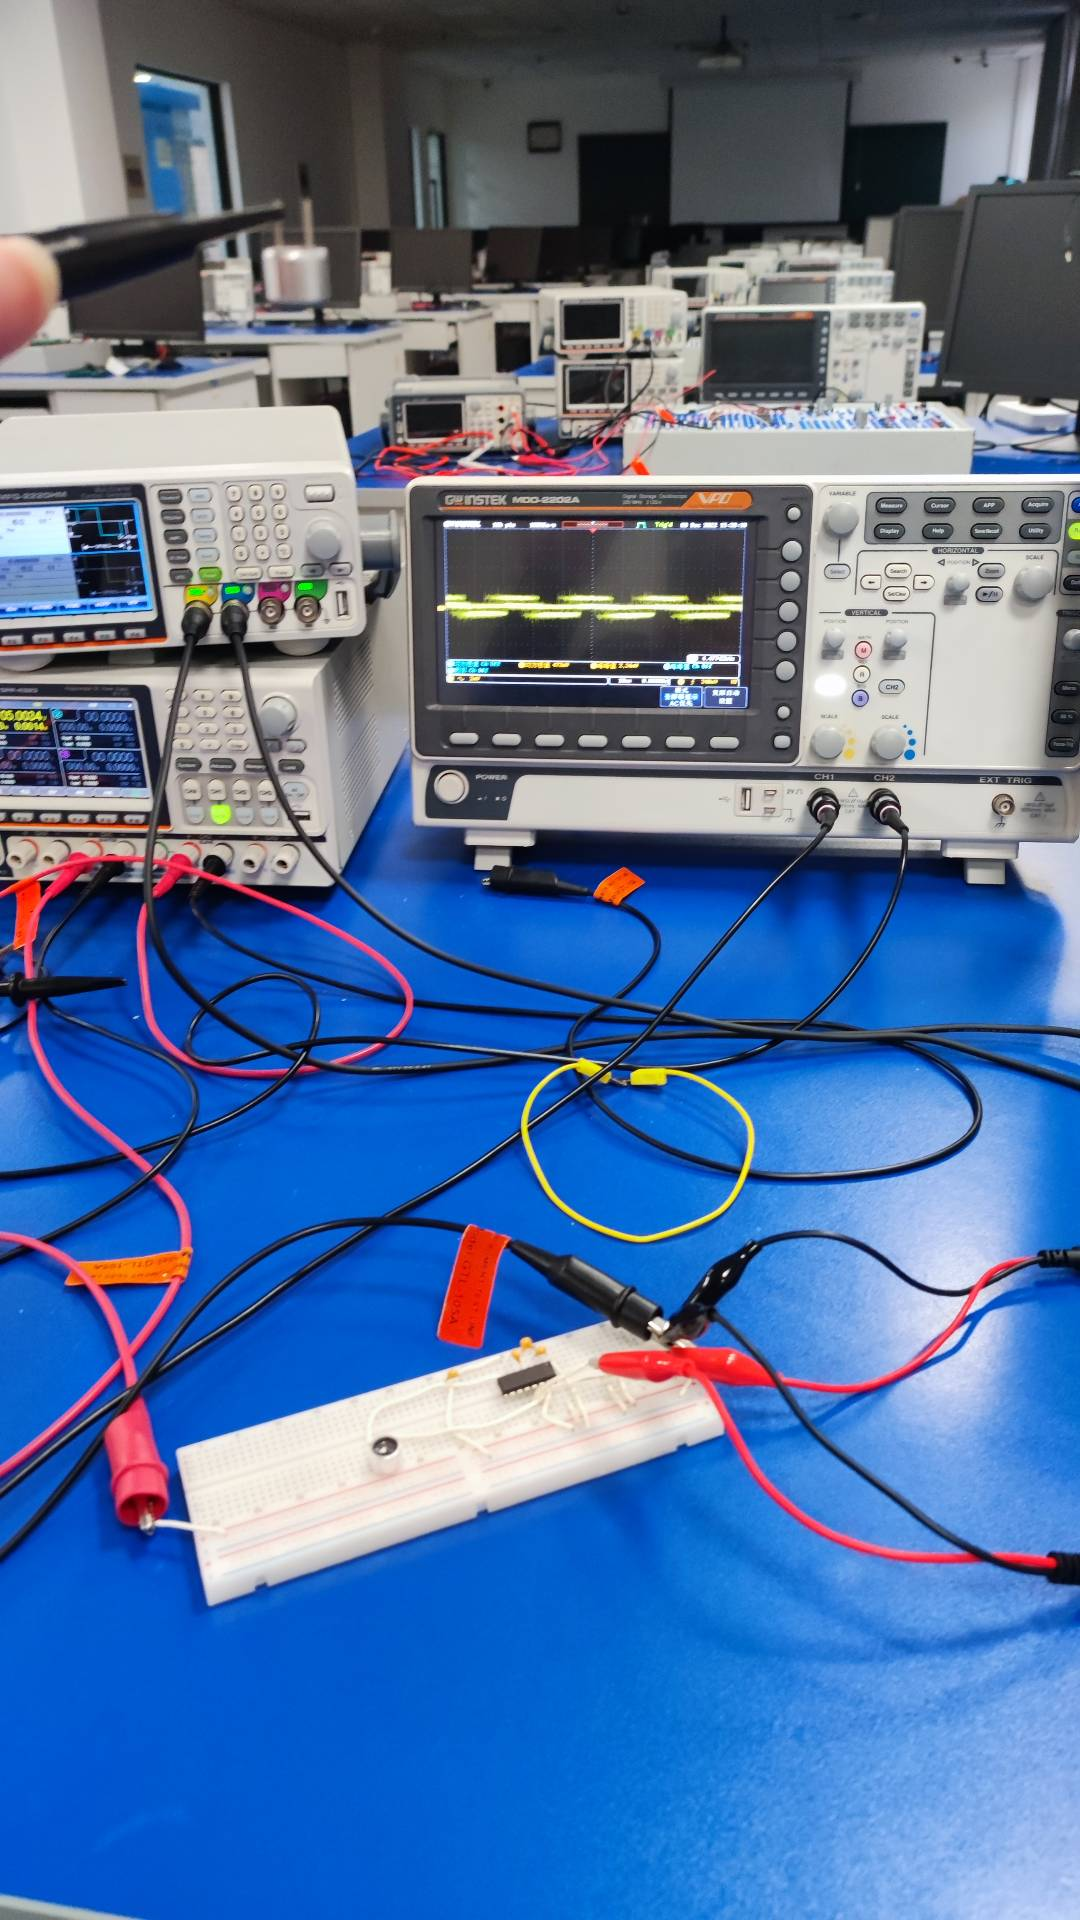
\includegraphics[width=0.9\linewidth]{图片/远距离}
	        \caption{远距离}
	        \label{mx232s}
	    \end{minipage}
	\end{figure}
	\section{摘要}
	我们实现了智能万用表的基本测量要求，在此基础上使用ESP8266模块实现了与服务器的TCP协议WIFI连接，并实现了时间显示功能和log记录功能。
	\subsection{使用器件表}
    \begin{figure}[h]
	    \centering
	    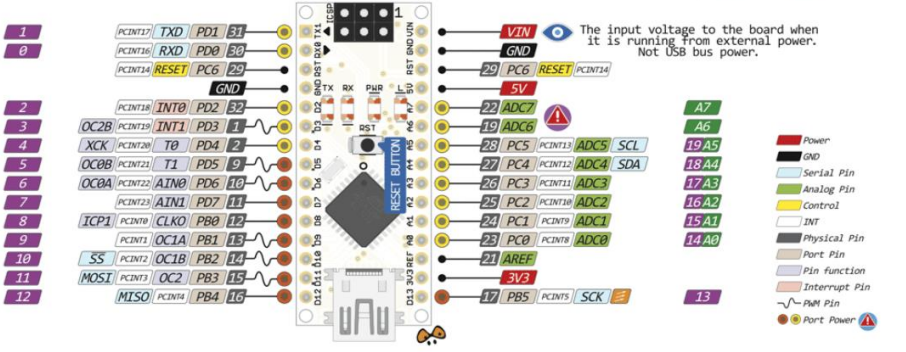
\includegraphics[width=0.8\linewidth]{图片/功能图}
	    \caption{Arduino NANO端口功能}
	    \label{nano}
	\end{figure}
    
    使用的器件有：Arduino Nano单片机若干，拓展板一块，Nokia5100 LCD显示器一块，杜邦线若干，开关一个，面包板两块，待测元件若干，ESP8266模块若干，6.7V可充电锂电池一块，服务器主机和路由器设备。   

	\section{原理说明}
	\subsection{电阻测量}
	\subsubsection{基本原理}
	已知阻值$R_0$,测量未知电阻$R_x$,可利用电阻分压规律来得到
	$R_x$:
	\begin{align*}
	    \frac{U_{R_x}}{V_{CC}}&=\frac{R_x}{R_x+R_0}\\
	    R_x&=\frac{U_{R_x}R_0}{V_{CC}-U_{R_x}}
	\end{align*}
	\par
	下面讨论如何选取适合的电阻值来配合未知电阻。
	\subsubsection{设计思路}
	利用已知两类阻值的电阻，我们要选取合适的阻值测量未知的$R_x$。对于阻值大的未知电阻，我们应当选择大值$R_0$,否则理论公式中$U_{R_x}$会接近于0，测量精确度低；小的未知电阻则应选小值$R_0$，否则理论公式中$U_{R_x}$会接近于$V_{CC}$,也使得测量不准。
	\par 我们可通过预测量的方式估计未知电阻的大小，再自动转入合适的档位进行精确的测量。当$R_x=35490.84\Omega$时两档所测$R_x$相对误差相等，在$V_{CC}=5V$时对应$R_0=680\Omega$的电压$U_{R_x}=4.818V$。则首先在输入端选用小的$R_0=680\Omega$,用一个ADC接口测量未知电阻端电压,若端电压$U_{R_x}>4.818V$ 则电阻阻值较大，换用$R_0=470k\Omega$档位进行测量。
	\subsection{电容测量}
	\subsubsection{基本原理}
	利用下图的一阶RC电路，我们能通过电路方程对于电容值进行测量
	\begin{figure}[H]
	    \centering
	    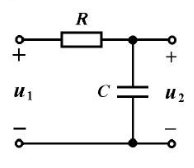
\includegraphics{图片/20221226144957.png}
	    \caption{基本一阶RC电路}
	    \label{fig:my_label}
	\end{figure}
	给予电压$U_1=V_{cc}$,我们利用下述公式求得电容值：
	\begin{equation*}
	    U_2=U_C=V_{cc}(1-e^\frac{t}{RC})
	\end{equation*}
	\par
	该公式主要用途是可通过充电时间与充电电压的关系来确定电容$C$的值。如对于
	小电容，为电路安全考虑不能充电太久，则采用“充电电压一定，测充电时间”的方式测定电容值；对于大电容，由于充电效率较低，可以采用“充电时间一定，测充电电压”的方式来测定电容值。在下一部分中将讨论方式的确定与参数的选取。
	\subsubsection{设计思路}
	对于测定电容端电压，方式类似电阻。同样选用一个ADC接口：
	\par 对于电阻选取，我们应尽可能让充电时间长，这样不论是充电时间一定时还是充电电压一定时，对数值的读取都会更为精确；当然充电时长也不应过长。则根据时间常数RC确定，对于大电容应当选取小电阻，小电容应当选取大电阻。
	\par 若认为t=5$\tau$时完成充放电，则只需测充电时间就能计算出电容C。由于Arduino时钟频率为16MHZ，时钟周期约为63ns，则$\tau$应至少在$\mu$s数量级才能有较好的测量效果。可先选取小电阻进行测量，若充电时间过短再切换大电阻。
	\subsection{三极管测量}
	\subsubsection{基本原理}
	\begin{figure}[H]
	    \centering
	    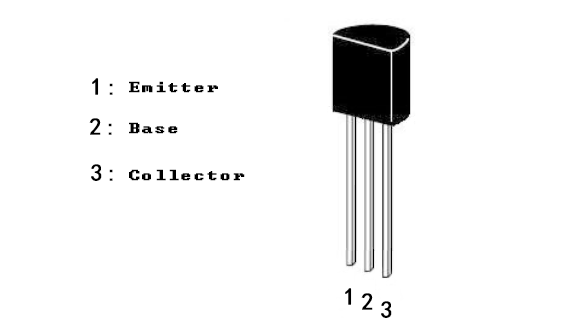
\includegraphics[scale=0.45]{图片/9013三极管.png}
	    \caption{三极管示意图}
	    \label{fig:my_label}
	\end{figure}
	三极管作为一个不对称元件，与之前的元件很大不同在于需要对不同端口的特性进行识别并做出选择。\subsubsection{双极管类型与电极的确定}
	首先我们应明确三极管的结构，对于一个双极晶体管，我们只可能从b极分别往c极和e极加电压时才有可能导通。并且对于PNP 型的管，b极应当是低电位；对于NPN型的管，b极应当是高电位。\par
	假设现有一枚NPN型双极管，我们可以对三级分别接入高电位进行b极的确定。当我们接高电压的极为b时，则两侧均能导通；若为c或e极，则两侧均截止。对于PNP管原理是一样的，但用的是低电位，同样，若接到b极则能检测到两侧导通，接到c或e极则一侧导通，另一侧截止。\par
	通过这样的测试，我们能确定出管子的类型以及其b极的位置。接下来我们应确定c，e极。根据三极管的物理特性，我们知道集电极具有较高的掺杂浓度，当给予的电压相同时，bc具有比be更小的电阻与更大的电流。故根据已确定的PNP(NPN),分别接低(高)电压，判断两端导通电流大者为c，小者为e。
	\subsubsection{参数$\beta$与$U_{be}$的测量}
	下面以NPN管为例说明参数的测量方式。下图是被采用的测量电路，
	\begin{figure}[H]
	    \centering
	    
\includegraphics[scale=0.8]{图片/4.png}
	    \caption{基本一阶RC电路}
	    \label{fig:my_label}
	\end{figure}
	其中$R_b=510k\Omega,R_c=680\Omega$（电阻阻值的选择是根据导通后两电阻的分压应当量级接近而进行的）根据有关模电知识计算可得：
	\begin{align*}
	    U_{BE}=V_{BQ}-V_E\\
	    \beta=\frac{V_E/R_e}{(V_{CC}-V_{BQ}/R_b}
	\end{align*}
	\par 对PNP管，测量方式与NPN管类似。
	\subsubsection{设计思路}
	对于工作在饱和区的三极管，有$V_b$与$V_e$的差约为0.3V~0.7V。对于NPN型三极管有$V_b$>$V_c$>$V_e$，PNP型三极管有$V_e$>$V_c$>$V_b$。在实际测量过程中可依次让一个端口接高电位，另外两个端口接低电位，观察三极管何时满足上述条件，再根据电压之间的关系就能测出三极管的端口信息。
	\section{仿真模拟}
	\begin{figure}[H]
	    \centering
	    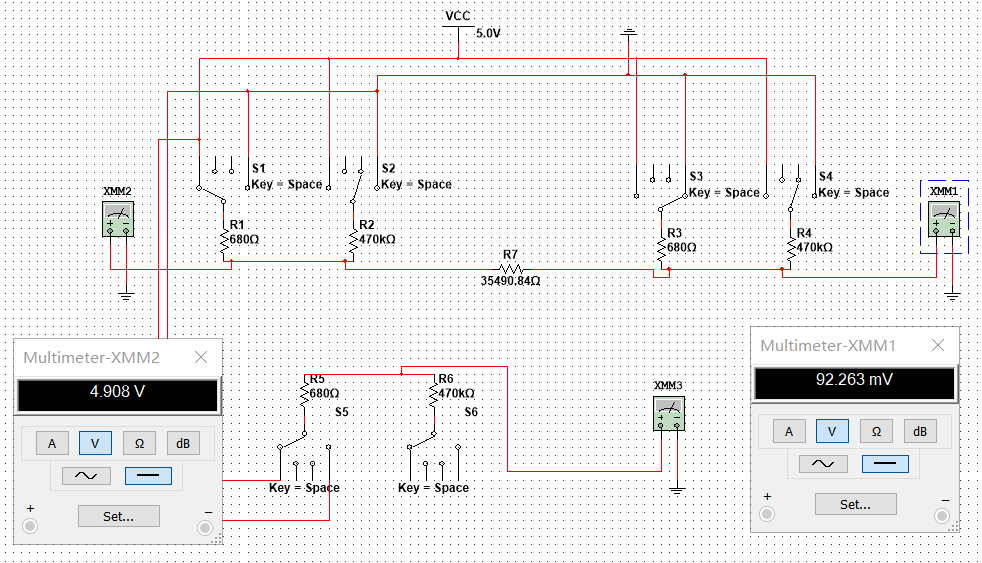
\includegraphics[scale=0.45]{图片/电阻仿真.png}
	    \caption{电阻测量电路}
	    \label{fig:my_label}
	\end{figure}
	\begin{figure}[H]
	    \centering
	    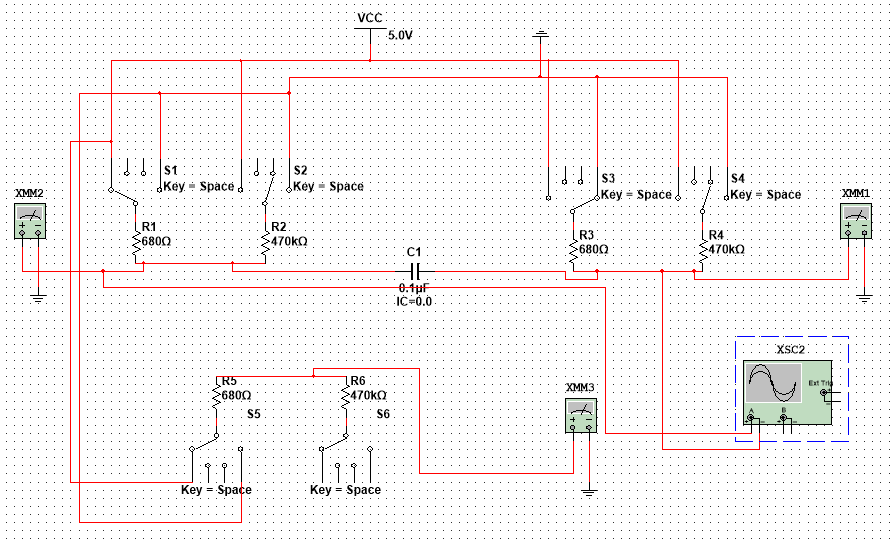
\includegraphics[scale=0.5]{图片/电容仿真电路.png}
	    \caption{电容测量电路}
	    \label{fig:my_label}
	\end{figure}
	\begin{figure}[H]
	    \centering
	    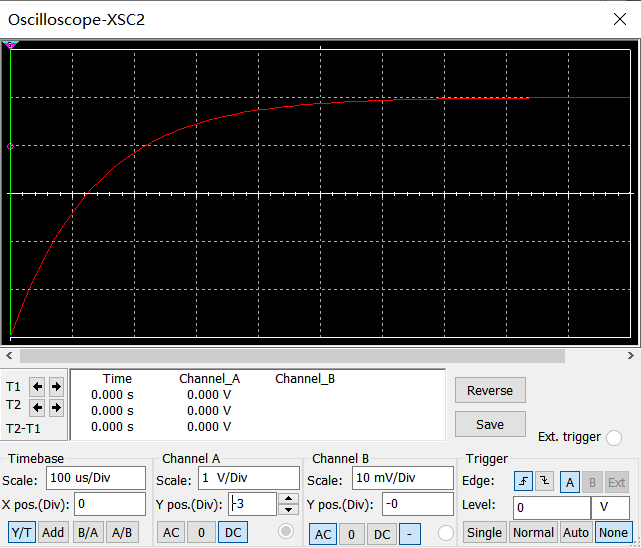
\includegraphics[scale=0.56]{图片/电容充电曲线.PNG}
	    \caption{电容充电曲线}
	    \label{fig:my_label}
	\end{figure}
	\begin{figure}[H]
	    \centering
	    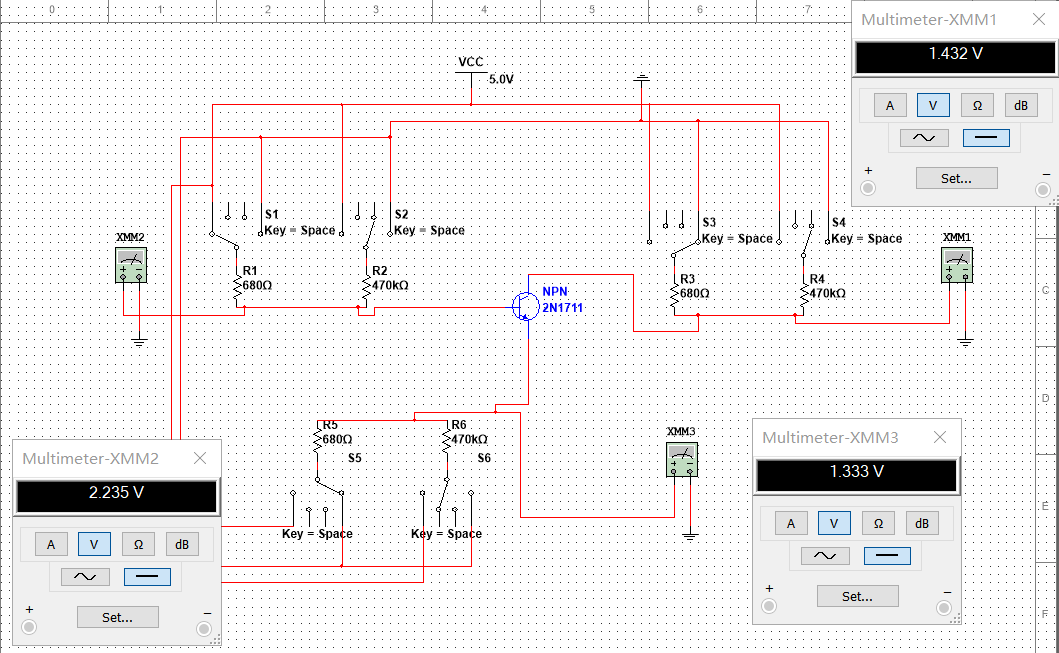
\includegraphics[scale=0.45]{图片/NPN.png}
	    \caption{NPN型三极管}
	 \end{figure}
	\begin{figure}[H]
	    \centering
	    \label{fig:my_label}
	     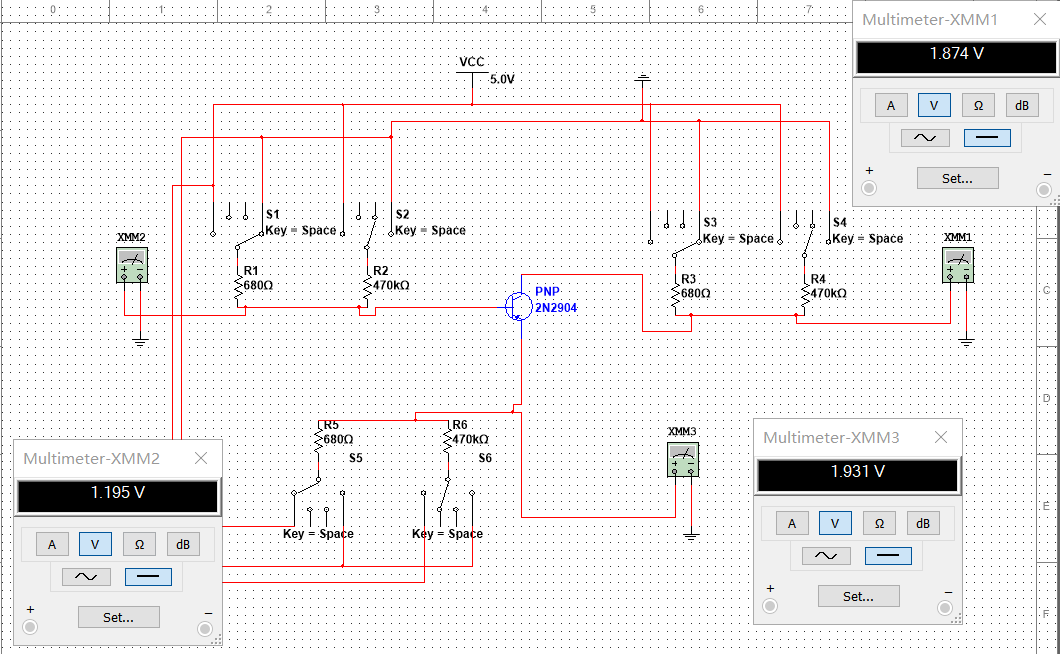
\includegraphics[scale=0.45]{图片/PNP.png}
	    \caption{PNP型三极管}
	\end{figure}
	\section{电路和代码实现}
	\subsection{基本功能}
	本作业中，所需实现的功能主要有：电阻参数的测量，电容参数的测量，三极管参数的测量。

	图\ref{re}是我们的成果实物图。
	
	\begin{figure}[h]
	    \centering
	    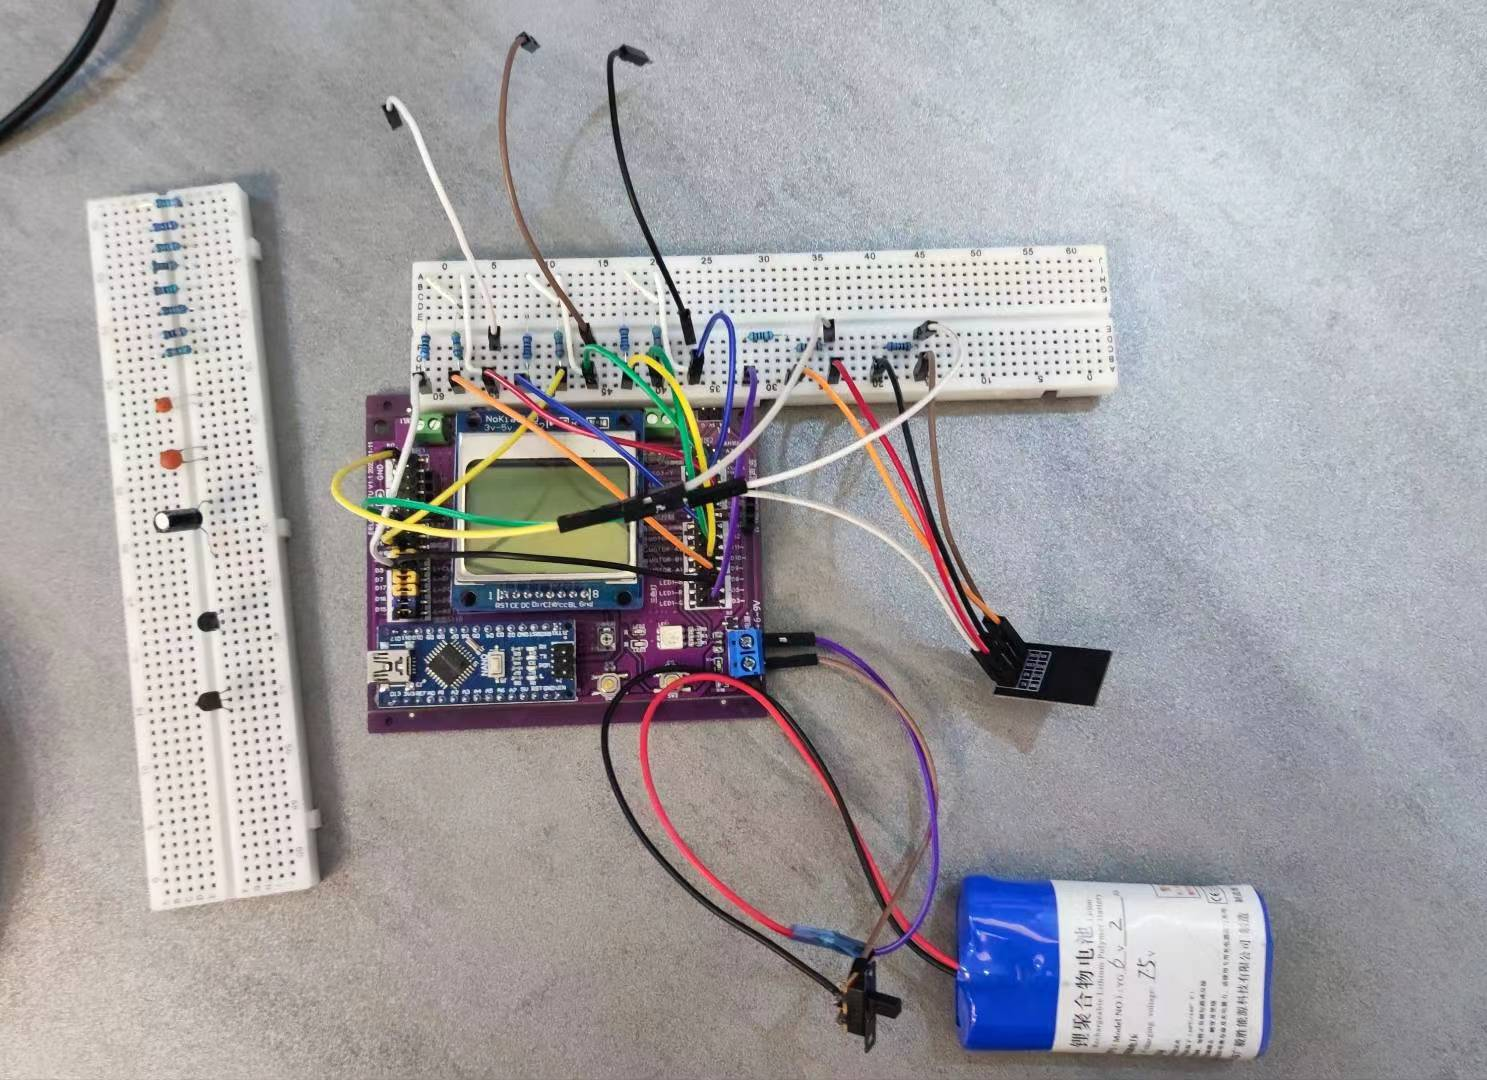
\includegraphics[width=0.6\linewidth]{图片/实物图}
	    \caption{成果实物图}
	    \label{re}
	\end{figure}
	
	主体部分使用了拓展板进行接线。拓展板仅作为接线柱和供电使用，我们没有使用拓展板的任何其他功能，包括屏幕跳线也是重新定义的。屏幕是原选题使用的LCD屏幕。
	
	此外，我们还使用了锂电池供电和无线网络模块，会在之后的部分进行说明。
	
	面板版上连接了通过杜邦线引出来的读写端口和电阻。单个测试节点包含一个具有ADC采样功能的端口和两个可写端口，其中可写端口分别连接680$\Omega$和470$k\Omega$的电阻，最后并联引出测试点。测试点电路如图\ref{tp}所示。由于三个测试点是对称的，我们将面板版上的连线也做到了对称和美观，电阻位置和测试点引线十分清晰。
	
	\begin{figure}[h]
	    \centering
	    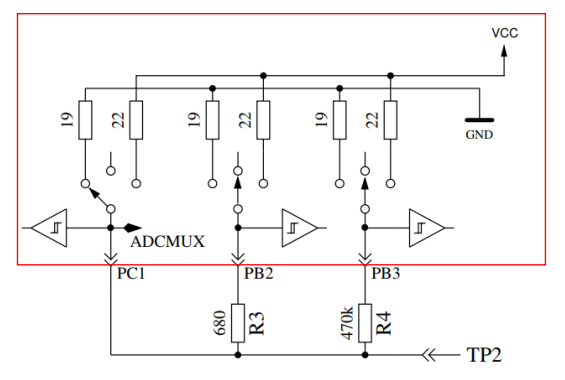
\includegraphics[width=0.4\linewidth]{图片/tp}
	    \caption{测试点电路图}
	    \label{tp}
	\end{figure}
	
	我们的端口定义如表\ref{port}所示。
	
	\begin{table}[h]
	    \centering
	    \caption{端口定义}
	    \label{port}
		\begin{tabular}{c|c|c}
			\hline\hline
			端口号 & 功能 & 用途 \\ \hline
            D14 & ADC0 & TP1读取 \\
            D8 & PB0 & TP1电平 \\ 
            D9 & PB1 & TP1电平 \\ 
            D15 & ADC1 & TP2读取 \\
            D12 & PB4 & TP2电平 \\ 
            D13 & PB5 & TP2电平 \\ 
            D16 & ADC2 & TP3读取 \\
            D10 & PB2 & TP3电平 \\ 
            D11 & PB3 & TP3电平 \\ 
            D6 & PD6 & 显示控制 \\
            D3 & PD3 & 8266TX \\
            D2 & PD2 & 8266RX \\ 
			 \hline \hline
		\end{tabular}
	\end{table}	 
	
	\subsection{电阻测量实现}
	如何确定测量使用的TP点将在控制部分阐述。此处均假设已知测试点信息和所需测量元件类型。
	
	实现电容的测量，首先假设电容较小。即：将470$k\Omega$连接的端口悬空，将680$\Omega$连接的端口电平写为一高一低，使用两个ADC端口的采样结果计算外接电阻上的电压差。ADC读取结果为一个10比特位表示的无符号整数，即取值在[0,1023]。最高电压为5V，通过简单的线性关系就可以得到电压的采样值。
	
	使用如下函数完成读取电压差值的操作。
\begin{lstlisting}[language=C]
// test the case for small resistance
double testRS(int x, int y, int cmd=1)
{
  setLow();
  pinMode(TP[x][ADC], INPUT);
  pinMode(TP[y][ADC], INPUT);
  pinMode(TP[x][Rl], INPUT);
  pinMode(TP[y][Rl], INPUT);
  pinMode(TP[x][Rs], OUTPUT);
  pinMode(TP[y][Rs], OUTPUT);
  digitalWrite(TP[x][Rs], HIGH);
  digitalWrite(TP[y][Rs], LOW);
  delay(5);
  int vinth=analogRead(TP[x][ADC]);
  int vintl=analogRead(TP[y][ADC]);
  if(abs(vinth+vintl-1023)>5 and cmd)
    return 114;
  double vdiff = (vinth-vintl)*5.0/1023;
  return vdiff;
}
\end{lstlisting}
	通过分压关系可以得到对应的电阻值。
	
	测量较大电阻时，换用大电阻进行分压即可。
	\subsection{电容测量实现}
	测量电容时，需要首先稳定两端电压为0。从此时开始计时，并将一端电压设为高电平。测量大电容是，选用小电阻，测量小电容时，使用大电阻。一段时间后，ADC采样获取电压差值达到某一设定好的电压，此时停止计时。时间长度为约10RC左右，以此计算电容值。具体充电时间与设定好的到达电压直接相关，与温度等其他因素也有关联。

    以下的代码可以用于测量较大电容。
\begin{lstlisting}
// large capacity
String testCL(int x, int y)
{ 
  setLow();
  disp(String("Mode: LC"), 0, 1); // Small C
  disp(String("Testing"), 0, 2);
  disp(String("Don't shift!"), 0, 3); // Warning
  pinMode(TP[x][ADC], INPUT);
  pinMode(TP[y][ADC], INPUT);
  pinMode(TP[x][Rl], INPUT); // use small R, the charge time is RC. If C is too small, charge time is small. This case goto TestCS to use larger R
  pinMode(TP[y][Rl], INPUT);
  pinMode(TP[x][Rs], OUTPUT);
  pinMode(TP[y][Rs], OUTPUT);
  int rcdv[200];
  String tmpS;
  int cnt=0;
  int vinth=analogRead(TP[x][ADC]);
  int vintl=analogRead(TP[y][ADC]);
  while(vinth>5 or vintl>5)
    vinth=analogRead(TP[x][ADC]), vintl=analogRead(TP[y][ADC]); // wait until q=0
  delay(10);
  long int Cstart=micros();
  digitalWrite(TP[x][Rs], HIGH);
  while(analogRead(TP[x][ADC])<1018 and micros()-Cstart<1000000)
      rcdv[max(cnt++/3,200)]=analogRead(TP[x][ADC]);
  long int tdiff=micros()-Cstart-116; // 116 is the base 
  tdiff=abs(tdiff);
  disp("            ", 0, 3);
  disp("Used "+String(tdiff)+"us",0,3);
  if(tdiff>900000)
  {
    disp("            ", 0, 0);
    disp("            ", 0, 1);
    disp("            ", 0, 2);
    disp("            ", 0, 3);
    return "Time LE";
  }
  if(tdiff<100)
    return testCS(x, y);
  else
  {
    espCom("plot cnt="+String(cnt)+"\r\n",10);
    for(register int i=0;i<200;++i)
      espCom(String(i)+","+String(rcdv[i])+",", 5);
  }
  return String(0.149*tdiff/680.0)+"uF  ";
}
\end{lstlisting}
	
	\subsection{三极管测量实现}
	首先扫描二极管，在两两端口加压寻找可以导通的端口，可以直接确定是PNP还是NPN型：如果是某一端口向另外两端导通，则为NPN；如果是两端向同一端口导通，则为PNP。其中，共同的端口为基极。在另外两端写入不同电平进行测量，根据原理公式，测得放大倍数较高的值为正偏放大倍数，较小为反偏放大倍数。
	
	以下代码实现了测量操作NPN三极管的操作。
\begin{lstlisting}
void testNPN(int b)
{
  setLow();
  disp(String("Mode: NPN"), 0, 1);
  pinMode(TP[1][ADC], INPUT);
  pinMode(TP[2][ADC], INPUT);
  pinMode(TP[3][ADC], INPUT);
  // first we suppose b+1 is e and b+2 is c
  int c=1+b%3, e=1+(b+1)%3;
  pinMode(TP[b][Rl], OUTPUT);
  pinMode(TP[c][Rs], OUTPUT);
  pinMode(TP[e][Rs], OUTPUT);
  digitalWrite(TP[b][Rl], HIGH);
  digitalWrite(TP[c][Rs], HIGH);
  digitalWrite(TP[e][Rs], LOW);
  int sw;
  if(not isValid((analogRead(TP[b][ADC])-analogRead(TP[e][ADC]))/1023.0*5.0)) // block
  {
    sw=c, c=e, e=sw;
    pinMode(TP[c][Rl], INPUT);
    pinMode(TP[e][Rl], INPUT);
    pinMode(TP[c][Rs], OUTPUT);
    pinMode(TP[e][Rs], OUTPUT);
    digitalWrite(TP[c][Rs], HIGH);
    digitalWrite(TP[e][Rs], LOW);
    if(not isValid((analogRead(TP[b][ADC])-analogRead(TP[e][ADC]))/1023.0*5.0))
    {
      disp("Invalid", 0, 2);
      delay(1000);
      return;
    }
  }
  disp("TP:e"+String(e)+"b"+String(b)+"c"+String(c), 0, 0);
  delay(50);
  double vb=analogRead(TP[b][ADC])/1023.0*5.0, vc=analogRead(TP[c][ADC])/1023.0*5.0, ve=analogRead(TP[e][ADC])/1023.0*5.0, vcc=5.0;
  // disp("TP:e"+String(analogRead(TP[e][ADC]))+"b"+String(analogRead(TP[b][ADC]))+"c"+String(analogRead(TP[c][ADC])), 0, 3);
  disp("beta="+String((vcc-vc)/680/((vcc-vb)/470000)), 0, 2);
  delay(500);
}
\end{lstlisting}
	
	\subsection{控制原理}
		控制函数重复代码多，仅在附录里给出。
		
		控制逻辑的基本要求是：涵盖所有可能的情况，并尽可能避免识别错误导致无法测量的情况。
		
		接下来阐述控制的具体逻辑：
		
		总体流程是判断三极管、判断小电阻、判断短路、判断电容（含断路）、判断大电阻、判断错误。
		\begin{enumerate}
		    \item 第一步进行三极管的判断，因为三极管测量时由于电压进行两两端口电压扫描。由于使用小电阻加电平，扫描时间耗时可以控制在35ms以内。扫描到上文所述的两个0.7V的导通电压，即进入三极管测量函数。如果不优先判断三极管，容易识别成分压为导通电压的电阻或识别为电容。测试三极管的主要时间消耗就是扫描，所以三极管可以秒测，显示停留一段时间方便读数。
		    \item 第二步测量小电阻。刚才已经测试了两两电压。如果分压在合理的范围，就直接计算输出小电阻值。在测量小电阻时，由于小电阻电压扫描很快，刷新率和灵敏度很高。几乎做到即插即测，拔掉瞬间回复空载。
		    \item 第三步测量电容。测量电容是扫描前面两两电压为0的点进行充放电测试首先进入大电容测试函数，如果瞬间充放电完成，说明电容过小换用大电阻进行小电容测试，如果依然过小，则其实是空载，输出空载。空载判断就是识别为一个十分小的电容。如果所有断路的测试点都是空载，那么就是空载情况，如果测到了电容值，则输出。为了避免插拔导致的电容充电开始，元件却重新插入了电阻中，导致无法充满，设置了最长充电时长。如果超时，输出Time LE。由于三极管已经排除，不会发生误识别。
		    
		    测试电容时，还需要讲采样点用数组保存以发送给服务器。实际测试时，发现使用局部变量，数组允许大小过小，而且发现电容的测试结果也受到数组大小明显影响。推测原因是寻址时间加长，导致判断充电完成的周期加长，最后一次测试导致的溢出时间增加，电容测试结果偏大。
		    \item 第四步，如果有短路点，则输出。短路的测试位置不是十分重要。
		    \item 第五步测试大电阻。这是因为大电阻测试需要设置更高的延时。测试发现，如果不进行延时，大电阻分压不能达到理论值，而延时后正常。讲大电阻测量放到最后，是考虑了系统的使用体验，否则测量其他元件时，需要等待大电阻完成扫描测试，耗时长。
		    \item 如果没有进入任何测试（实际上没有发生这样的事），输出错误并重启。
		\end{enumerate}
		
	\subsection{附加功能}
	\begin{itemize}
	\item{电池}
	
	我们使用拓展板进行供电，我在上面焊接了电池和锂电池，可以实现可充电、可开关的真无线万用表。
    \item{显示}
    
	我们使用了国外大佬实现的NOKIA5110\_TEXT库。该库的功能有在指定位置显示字符和字符串。理论上该库支持图像，但经过长时间实验发现该库对点阵图进行了重编码，故启动动画没有使用图像。使用不断变化位置的字符串显示了开机欢迎动画。开机后，显示器上方根据模式显示当前模式、测试结果、提示和警告、测试点信息。测试点信息是三极管的ebc极位置或者电容电阻的两端。提示会显示电容测试中，不要拔掉等信息。测试电容时，还会输出充电时间。三极管和电容测试结果有读数延时，小电阻测量时显示器会以高刷新率刷新，大电阻时刷新率降低。
	
	如果连接了服务器，屏幕下方会显示当前时间，并且会和测试结果同步刷新。
	\item 无线模块
	
	如图\ref{8266}连接了无线模块ESP8266模块实现WIFI连接。使用如下代码实现网络连接。其中，esoCom函数在附录中，实现的功能是单片机将信息写给8266，并收取一定时间内的返回信息。
    \begin{figure}[h]
	    \centering
	    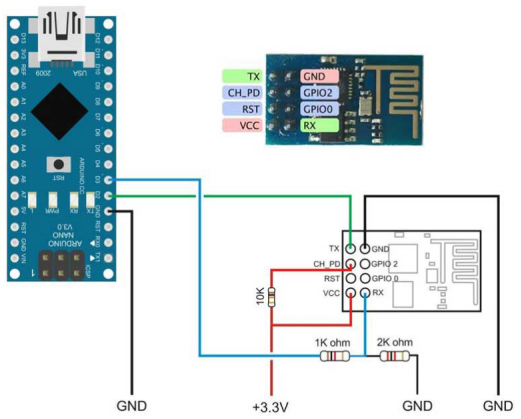
\includegraphics[width=0.4\linewidth]{图片/8266}
	    \caption{WIFI模块连线}
	    \label{8266}
	\end{figure}	
	
	
	\begin{lstlisting}
  // wifi connection
  Serial.begin(baud);
  esp.begin(baud);
  delay(5000);
  code below will be remembered inside esp8266
  espCom(F("AT+SAVETRANSLINK=1,\"192.168.1.9\",2333,\"TCP\"\r\n"), 2000);
  espCom(F("AT+CWMODE=1\r\n"), 2000);
  espCom(F("AT+RST\r\n"), 2000);
  espCom(F("AT+CWJAP=\"CMCC-SJTU\",\"Ww331811\"\r\n"), 10000);
  espCom(F("AT+CIPSTART=\"TCP\",\"192.168.1.9\",2333\r\n"), 10000);
  espCom(F("AT+CIPMODE=1\r\n"), 2000);
  espCom(F("AT+CIPSEND\r\n"), 2000);
  rt = espCom("Client Started.\r\n", 500);
	\end{lstlisting}
	
	在ESP8266中刷入标准AT固件，如上的AT指令只需执行一次，设置了8266储存连接信息，并且上电开启透传模式，即仅作为转发器。每次识别，单片机将缓存发送给服务器，服务器发回当前时间字符串。
	
	服务器使用python实现，使用WIFI连接，可以实现类似共享单车（共享单车一般使用蓝牙）的远程连接。使用TCP协议，可以防止信息丢失。具有多路连接，将万用表与手机进行连接，连接多个万用表等功能（即实现了多线程连接）。服务器收取缓存后，将log写在服务器本地。如果发现万用表测试了一次电容，就尝试绘图。但是发现，由于记录需要时间，实际测试的第一个记录点电压已经到了较高的位置，绘图过于离散，于是提交的代码中取消了该功能。
	
	结合服务器和本期储存，以及拓展板上的按钮，还可以实现历史记录调取的功能，菜单指定模式等，思路简单，没有给出实现。
	
	\subsection{精度和BUG分析}
	测试结果于附件表格给出。电阻测试精度较高。在测试了足够多的电阻后，使用理想计算公式图线存在系统偏差，在原式中添加参数整体移动了图线使之准确。可惜的是，由于是电阻数量不够多，无法细调。为了避免凑数嫌疑，保留了一定误差。电容存在类似情况。电容误差还与代码量有关联，发现增删无关代码影响电容测试结果，匪夷所思。推测是由于采用了自己购买的芯片，时钟不稳定。实际测试时，发现时钟差到288ns时才会发生跳变，可能也与之有关。这也影响电容的准确程度。三极管按照理想电路进行了测试，由于没有标准测试仪，我们本着诚实的态度，输出了于参数误差极大的放大倍数，没有进行修改。但是，我们测试了温度影响下的放大倍数变化，证明我们测试的结果确实与放大倍数正相关。
	
	在测试过程中，随意插拔，可能导致显示屏幕花屏。但是从服务器运行状态上看，测试在正常进行，推测为国外大佬显示器代码bug。此外，也有小概率发生单片机死机重启，但比较难以触发，故不纠其原因。

    \end{itemize}
    
	\section{团队分工}
	王凯灵：前期实现了超声波电路。设计实现了万用表电路和代码以及拓展功能，报告撰写相应部分。
	
	代铭波：元件测量仪部分理论和设计思路推导，模拟仿真，报告撰写相关部分。
	
	张杭磊：原理部分的撰写，报告内容与图片的排版。
\lstset{
	numbers=left,
	numberstyle=\color[RGB]{0,192,192},
	backgroundcolor=\color[RGB]{245,245,244},
	basicstyle=\ttfamily\small,
	breakatwhitespace=false,
	breaklines=true,
	captionpos=b,
	commentstyle=\color{gray},
	directivestyle=\color{blue},
	extendedchars=false,
	framexleftmargin=8mm,
	framexrightmargin=8mm,
	framerule=0pt,
	keywordstyle=\color{blue}\bfseries,
	morekeywords={*,define,*,include...},
	numbersep=5pt,
	rulesepcolor=\color{red!20!green!20!blue!20},
	showspaces=false,
	showstringspaces=false,
	showtabs=false,
	stringstyle=\color{purple},
	tabsize=4,
	title=\lstname
    frame=tb,
	language=Python,
	aboveskip=3mm,
	belowskip=3mm,
	showstringspaces=false,
	columns=flexible,
	breaklines=true,
	breakatwhitespace=true,
}

\section{附录}
\subsection{嵌入式代码}
\lstset{
	language=[ANSI]{C},
	numbers=left,
	numberstyle=\color[RGB]{0,192,192},
	backgroundcolor=\color[RGB]{245,245,244},
	basicstyle=\ttfamily\small,
	breakatwhitespace=false,
	breaklines=true,
	captionpos=b,
	commentstyle=\color{gray},
	directivestyle=\color{blue},
	extendedchars=false,
	framexleftmargin=8mm,
	framexrightmargin=8mm,
	framerule=0pt,
	keywordstyle=\color{blue}\bfseries,
	morekeywords={*,define,*,include...},
	numbersep=5pt,
	rulesepcolor=\color{red!20!green!20!blue!20},
	showspaces=false,
	showstringspaces=false,
	showtabs=false,
	stringstyle=\color{purple},
	tabsize=4,
	title=\lstname
	}
\begin{lstlisting}
// define the LCD screen
#include <NOKIA5110_TEXT.h>
NOKIA5110_TEXT display(15, 16, 17, 7, 6);
#define inverse  false
#define UseDefaultFont  false
#define contrast 0xBF // default is 0xBF set in LCDinit, Try 0xB1(good @ 3.3V) or 0xBF if your display is too dark
#define bias 0x13 // LCD bias mode 1:48: Try 0x13 or 0x14
#define cd display.LCDClear();
// define the 8266 module
#include <SoftwareSerial.h>
SoftwareSerial esp(2, 3);
uint32_t baud = 115200;
String rt = "";
// control bits for testpoints
int TP[4][3]{0, 0, 0, 8, 9, 14, 12, 13, 19, 10, 11, 18};
#define Rs 0 // small R = 680 Ohm
#define Rl 1 // large R = 470 kOhm
#define ADC 2 // ADC input(PCx) 

#define msg String(rcd[0][0][1])+","+String(rcd[0][0][2])+","+String(rcd[0][1][0])+","+String(rcd[0][1][2])+","+String(rcd[0][2][0])+","+String(rcd[0][2][1])+","+String(rcd[1][0][1])+","+String(rcd[1][0][2])+","+String(rcd[1][1][0])+","+String(rcd[1][1][2])+","+String(rcd[1][2][0])+","+String(rcd[1][2][1])+"\r\n"

void setup()
{
  // screen init and boot effect
  display.LCDInit(inverse, contrast, bias); //initialize
  cd //clear whole screen
  
  // wifi connection
  Serial.begin(baud);
  esp.begin(baud);
  delay(5000);
  // code below will be remembered inside esp8266
  // espCom(F("AT+SAVETRANSLINK=1,\"192.168.1.9\",2333,\"TCP\"\r\n"), 2000);
  // espCom(F("AT+CWMODE=1\r\n"), 2000);
  // espCom(F("AT+RST\r\n"), 2000);
  // espCom(F("AT+CWJAP=\"CMCC-SJTU\",\"Ww331811\"\r\n"), 10000);
  // espCom(F("AT+CIPSTART=\"TCP\",\"192.168.1.9\",2333\r\n"), 10000);
  // espCom(F("AT+CIPMODE=1\r\n"), 2000);
  // espCom(F("AT+CIPSEND\r\n"), 2000);
  onboot_notice();
  rt = espCom("Client Started.\r\n", 500);
}

void loop()
{
  if(rt[0]=='t')
    rt[0] = ' ', disp(rt+" ", 0, 4);
  rt = espCom(autoSelect(), 333);
  
}

// simple display controller
void disp(String s, int X, int Y)
{
  display.LCDgotoXY(X, Y); // (go to (X , Y) (0-84 columns, 0-5 blocks)
  display.LCDString(&s[0]); //print
}

// onboot animation♂
void onboot_notice()
{
  for(register int i=0; i<6; ++i)
  {
    disp("114", 15, i);
    disp("514", 55, 5-i);
    delay(300);
  }
  cd
  disp("Welcome", 20, 2);
  disp("to use", 25, 3);
  disp("LOPING151", 15, 5);
  delay(3000);
  cd
  display.LCDgotoXY(0, 0);
  display.LCDString("Connecting");
  display.LCDgotoXY(0, 1);
  display.LCDString("to server");
  display.LCDgotoXY(0, 2);
  delay(2000);
  cd
}

// send command or data to the server
String espCom(String command, const int timeout)
{
  String inData = "";
  esp.print(command);
  long int time = millis();
  while ( (time + timeout) > millis())
  {
    while (esp.available())
    {
      char c = esp.read();
      inData += c;
    }
  }
  return inData;
}

// set all pin Low before each test
void setLow()
{
  for(register int i=1;i<=3;++i)
    for(register int j=0;j<=2;++j)
      pinMode(TP[i][j], INPUT);
}

// test the case for small resistance
double testRS(int x, int y, int cmd=1)
{
  setLow();
  pinMode(TP[x][ADC], INPUT);
  pinMode(TP[y][ADC], INPUT);
  pinMode(TP[x][Rl], INPUT);
  pinMode(TP[y][Rl], INPUT);
  pinMode(TP[x][Rs], OUTPUT);
  pinMode(TP[y][Rs], OUTPUT);
  digitalWrite(TP[x][Rs], HIGH);
  digitalWrite(TP[y][Rs], LOW);
  delay(5);
  int vinth=analogRead(TP[x][ADC]);
  int vintl=analogRead(TP[y][ADC]);
  if(abs(vinth+vintl-1023)>5 and cmd)
    return 114;
  double vdiff = (vinth-vintl)*5.0/1023;
  return vdiff;
}

// test the case for large resistance
double testRL(int x, int y)
{
  setLow();
  pinMode(TP[x][ADC], INPUT);
  pinMode(TP[y][ADC], INPUT);
  pinMode(TP[x][Rs], INPUT);
  pinMode(TP[y][Rs], INPUT);
  pinMode(TP[x][Rl], OUTPUT);
  pinMode(TP[y][Rl], OUTPUT);
  digitalWrite(TP[x][Rl], HIGH);
  digitalWrite(TP[y][Rl], LOW);
  delay(50);
  int vinth=analogRead(TP[x][ADC]);
  int vintl=analogRead(TP[y][ADC]);
  if(vinth<850)
    delay(200);
  else
    return 514;
  vinth=analogRead(TP[x][ADC]);
  vintl=analogRead(TP[y][ADC]);
  if(abs(vinth+vintl-1023)>15)
    return 514;
  double vdiff = (vinth-vintl)*5.0/1023;
  return vdiff;
}

// large capacity
String testCL(int x, int y)
{ 
  setLow();
  disp(String("Mode: LC"), 0, 1); // Small C
  disp(String("Testing"), 0, 2);
  disp(String("Don't shift!"), 0, 3); // Warning
  pinMode(TP[x][ADC], INPUT);
  pinMode(TP[y][ADC], INPUT);
  pinMode(TP[x][Rl], INPUT); // use small R, the charge time is RC. If C is too small, charge time is small. This case goto TestCS to use larger R
  pinMode(TP[y][Rl], INPUT);
  pinMode(TP[x][Rs], OUTPUT);
  pinMode(TP[y][Rs], OUTPUT);
  int rcdv[200];
  String tmpS;
  int cnt=0;
  int vinth=analogRead(TP[x][ADC]);
  int vintl=analogRead(TP[y][ADC]);
  while(vinth>5 or vintl>5)
    vinth=analogRead(TP[x][ADC]), vintl=analogRead(TP[y][ADC]); // wait until q=0
  delay(10);
  long int Cstart=micros();
  digitalWrite(TP[x][Rs], HIGH);
  while(analogRead(TP[x][ADC])<1018 and micros()-Cstart<1000000)
      rcdv[max(cnt++/3,200)]=analogRead(TP[x][ADC]);
  long int tdiff=micros()-Cstart-116; // 116 is the base 
  tdiff=abs(tdiff);
  disp("            ", 0, 3);
  disp("Used "+String(tdiff)+"us",0,3);
  if(tdiff>900000)
  {
    disp("            ", 0, 0);
    disp("            ", 0, 1);
    disp("            ", 0, 2);
    disp("            ", 0, 3);
    return "Time LE";
  }
  if(tdiff<100)
    return testCS(x, y);
  else
  {
    espCom("plot cnt="+String(cnt)+"\r\n",10);
    for(register int i=0;i<200;++i)
      espCom(String(i)+","+String(rcdv[i])+",", 5);
  }
  return String(0.149*tdiff/680.0)+"uF  ";
}

// small capacity
String testCS(int x, int y) 
{  
  setLow();
  disp(String("Mode: SC"), 0, 1); // Large C
  pinMode(TP[x][ADC], INPUT);
  pinMode(TP[y][ADC], INPUT);
  pinMode(TP[x][Rs], INPUT);
  pinMode(TP[y][Rs], INPUT);
  pinMode(TP[x][Rl], OUTPUT);
  pinMode(TP[y][Rl], OUTPUT);
  int vinth=analogRead(TP[x][ADC]);
  int vintl=analogRead(TP[y][ADC]);
  while(vinth>2 or vintl>2)
    vinth=analogRead(TP[x][ADC]), vintl=analogRead(TP[y][ADC]); // wait until q=0
  long int Cstart=micros();
  digitalWrite(TP[x][Rl], HIGH);
  while(analogRead(TP[x][ADC])<1020 and micros()-Cstart<344);
  long int tdiff=micros()-Cstart-344;
  tdiff=abs(tdiff);
  disp("            ", 0, 3);
  disp("Used "+String(tdiff)+"us",0,3);
  if(tdiff>900000)
  {
    disp("            ", 0, 0);
    disp("            ", 0, 1);
    disp("            ", 0, 2);
    disp("            ", 0, 3);
    return "Time LE";
  }
  if(tdiff<220)
  {
    disp("            ", 0, 0);
    disp("            ", 0, 1);
    disp("            ", 0, 2);
    disp("            ", 0, 3);
    disp("Empty load", 0, 0);
    delay(500);
    return "";
  }
  return String(0.1*tdiff/470.0*1000)+"pF  ";
}

// judge if the voltage is valid for triod
bool isValid(double x)
{
  return x>0.4 and x<1.2;
}

void testNPN(int b)
{
  setLow();
  disp(String("Mode: NPN"), 0, 1);
  pinMode(TP[1][ADC], INPUT);
  pinMode(TP[2][ADC], INPUT);
  pinMode(TP[3][ADC], INPUT);
  // first we suppose b+1 is e and b+2 is c
  int c=1+b%3, e=1+(b+1)%3;
  pinMode(TP[b][Rl], OUTPUT);
  pinMode(TP[c][Rs], OUTPUT);
  pinMode(TP[e][Rs], OUTPUT);
  digitalWrite(TP[b][Rl], HIGH);
  digitalWrite(TP[c][Rs], HIGH);
  digitalWrite(TP[e][Rs], LOW);
  int sw;
  if(not isValid((analogRead(TP[b][ADC])-analogRead(TP[e][ADC]))/1023.0*5.0)) // block
  {
    sw=c, c=e, e=sw;
    pinMode(TP[c][Rl], INPUT);
    pinMode(TP[e][Rl], INPUT);
    pinMode(TP[c][Rs], OUTPUT);
    pinMode(TP[e][Rs], OUTPUT);
    digitalWrite(TP[c][Rs], HIGH);
    digitalWrite(TP[e][Rs], LOW);
    if(not isValid((analogRead(TP[b][ADC])-analogRead(TP[e][ADC]))/1023.0*5.0))
    {
      disp("Invalid", 0, 2);
      delay(1000);
      return;
    }
  }
  disp("TP:e"+String(e)+"b"+String(b)+"c"+String(c), 0, 0);
  delay(50);
  double vb=analogRead(TP[b][ADC])/1023.0*5.0, vc=analogRead(TP[c][ADC])/1023.0*5.0, ve=analogRead(TP[e][ADC])/1023.0*5.0, vcc=5.0;
  // disp("TP:e"+String(analogRead(TP[e][ADC]))+"b"+String(analogRead(TP[b][ADC]))+"c"+String(analogRead(TP[c][ADC])), 0, 3);
  disp("beta="+String((vcc-vc)/680/((vcc-vb)/470000)), 0, 2);
  delay(500);
}

void testPNP(int b)
{
  setLow();
  disp(String("Mode: PNP"), 0, 1);
  pinMode(TP[1][ADC], INPUT);
  pinMode(TP[2][ADC], INPUT);
  pinMode(TP[3][ADC], INPUT);
  // first we suppose b+1 is e and b+2 is c
  int c=1+b%3, e=1+(b+1)%3;
  pinMode(TP[b][Rl], OUTPUT);
  pinMode(TP[c][Rs], OUTPUT);
  pinMode(TP[e][Rs], OUTPUT);
  digitalWrite(TP[b][Rl], LOW);
  digitalWrite(TP[c][Rs], LOW);
  digitalWrite(TP[e][Rs], HIGH);
  int sw;
  if(not isValid(-(analogRead(TP[b][ADC])-analogRead(TP[e][ADC]))/1023.0*5.0)) // block
  {
    sw=c, c=e, e=sw;
    pinMode(TP[c][Rl], INPUT);
    pinMode(TP[e][Rl], INPUT);
    pinMode(TP[c][Rs], OUTPUT);
    pinMode(TP[e][Rs], OUTPUT);
    digitalWrite(TP[c][Rs], LOW);
    digitalWrite(TP[e][Rs], HIGH);
    if(not isValid(-(analogRead(TP[b][ADC])-analogRead(TP[e][ADC]))/1023.0*5.0))
    {
      disp("Invalid", 0, 2);
      delay(1000);
      return;
    }
  }
  disp("TP:e"+String(e)+"b"+String(b)+"c"+String(c), 0, 0);
  delay(50);
  double vb=analogRead(TP[b][ADC])/1023.0*5.0, vc=analogRead(TP[c][ADC])/1023.0*5.0, ve=analogRead(TP[e][ADC])/1023.0*5.0, vcc=5.0;
  // disp("TP:e"+String(analogRead(TP[e][ADC]))+"b"+String(analogRead(TP[b][ADC]))+"c"+String(analogRead(TP[c][ADC])), 0, 3);
  disp("beta="+String(vc/680/(vb/470000)), 0, 2);
  delay(500);
}

// do tests and auto select the mode
String autoSelect()
{  
  disp("            ", 0, 0);
  disp("            ", 0, 1);
  disp("            ", 0, 2);
  disp("            ", 0, 3);
   
  double rcdt[3][3]{};
  for(register int i=0;i<9;++i)
    if(i%3!=i/3)
      rcdt[i/3][i%3]=testRS(i/3+1, i%3+1, 0);
  // Cases for Triode
  if(isValid(rcdt[1][0]) and isValid(rcdt[2][0]))
  {
    testPNP(1);
    return "-1\r\n";
  }  
  if(isValid(rcdt[0][1]) and isValid(rcdt[2][1]))
  {
    testPNP(2);
    return "-1\r\n";
  }
  if(isValid(rcdt[0][2]) and isValid(rcdt[1][2]))
  {
    testPNP(3);
    return "-1\r\n";
  }
  if(isValid(rcdt[0][1]) and isValid(rcdt[0][2]))
  {
    testNPN(1);
    return "-1\r\n";
  }
  if(isValid(rcdt[1][0]) and isValid(rcdt[1][2]))
  {
    testNPN(2);
    return "-1\r\n";
  }
  if(isValid(rcdt[2][0]) and isValid(rcdt[2][1]))
  {
    testNPN(3);
    return "-1\r\n";
  }
  
  double rcd[2][3][3]{}; // rcd[0] records the results for testRS and rcd[1] for testRL.

  // Cases for R
  for(register int i=0;i<9;++i)
    if(i%3!=i/3)
    {
      rcd[0][i/3][i%3]=testRS(i/3+1, i%3+1);
      if(rcd[0][i/3][i%3]>=0.2 and rcd[0][i/3][i%3]<4.5)
      {
        disp(String("TP on ")+String(i/3+1)+String("-")+String(i%3+1), 0, 0);
        disp(String("Mode: SR"), 0, 1); // Small R
        disp(String(1.035*1360*rcd[0][i/3][i%3]/(5-rcd[0][i/3][i%3]))+String(" Ohm"), 0, 2);
        return msg;
      }
    }

  // Cases for short
  if(rcd[0][0][1]<0.1 or rcd[0][0][2]<0.1 or rcd[0][1][2]<0.1 or rcd[0][1][0]<0.1 or rcd[0][2][0]<0.1 or rcd[0][2][1]<0.1)
  {
    disp(String("Short"),0, 0), delay(2000);
    return msg;
  }

  for(register int i=0;i<9;++i)
    if(i%3!=i/3)
    {
      rcd[1][i/3][i%3]=testRL(i/3+1, i%3+1);
      if(rcd[1][i/3][i%3]>=0.1 and rcd[1][i/3][i%3]<=4.8)
      {
        disp(String("TP on ")+String(i/3+1)+String("-")+String(i%3+1), 0, 0);
        disp(String("Mode: LR"), 0, 1); // Large R
        disp(String(-8+1.233*940*rcd[1][i/3][i%3]/(5-rcd[1][i/3][i%3]))+String(" kOhm"), 0, 2);
        return msg;
      }
    }
    
  // Cases for C
  if((rcd[0][0][1]>4.5 or rcd[0][1][0]>4.5) and (max(rcd[0][0][1], rcd[0][1][0])>=max(rcd[0][0][2], rcd[0][2][0])) and (max(rcd[0][0][1], rcd[0][1][0])>=max(rcd[0][1][2], rcd[0][2][1])))
    {
      disp(String("TP on ")+String(1)+String("-")+String(2), 0, 0);
      String resultC = testCL(1, 2);
      if(resultC!="")
      {
        disp(resultC, 0, 2);
        delay(2000);
        cd
      }
      return msg;
    }
  if((rcd[0][0][2]>4.5 or rcd[0][2][0]>4.5) and (max(rcd[0][0][2], rcd[0][2][0])>=max(rcd[0][0][1], rcd[0][1][0])) and (max(rcd[0][0][2], rcd[0][2][0])>=max(rcd[0][1][2], rcd[0][2][1])))
    {
      disp(String("TP on ")+String(1)+String("-")+String(3), 0, 0);
      String resultC = testCL(1, 3);
      if(resultC!="")
      {
        disp(resultC, 0, 2);
        delay(2000);
        cd
      }
      return msg;
    }
  if((rcd[0][1][2]>4.5 or rcd[0][2][1]>4.5) and (max(rcd[0][1][2], rcd[0][2][1])>=max(rcd[0][0][2], rcd[0][2][0])) and (max(rcd[0][1][2], rcd[0][2][1])>=max(rcd[0][0][1], rcd[0][1][0])))
    {
      disp(String("TP on ")+String(2)+String("-")+String(3), 0, 0);
      String resultC = testCL(2, 3);
      if(resultC!="")
      {
        disp(resultC, 0, 2);
        delay(2000);
        cd
      }
      return msg;
    }


  // shouldn't reach here
  cd
  disp("Error", 0, 0);
  delay(5000);
  return msg;
}
\end{lstlisting}
\section{服务器端代码}
\lstset{
	numbers=left,
	numberstyle=\color[RGB]{0,192,192},
	backgroundcolor=\color[RGB]{245,245,244},
	basicstyle=\ttfamily\small,
	breakatwhitespace=false,
	breaklines=true,
	captionpos=b,
	commentstyle=\color{gray},
	directivestyle=\color{blue},
	extendedchars=false,
	framexleftmargin=8mm,
	framexrightmargin=8mm,
	framerule=0pt,
	keywordstyle=\color{blue}\bfseries,
	morekeywords={*,define,*,include...},
	numbersep=5pt,
	rulesepcolor=\color{red!20!green!20!blue!20},
	showspaces=false,
	showstringspaces=false,
	showtabs=false,
	stringstyle=\color{purple},
	tabsize=4,
	title=\lstname,
    frame=tb,
	language=Python,
	aboveskip=3mm,
	belowskip=3mm,
	showstringspaces=false,
	columns=flexible,
	breaklines=true,
	breakatwhitespace=true,
}
\begin{lstlisting}
import socket
import threading
import matplotlib.pyplot as plt
from time import sleep, time, strftime, localtime
from sys import exit
import numpy as np
from csv import reader

plt.rcParams['font.sans-serif'] = ['SimHei']  # 表格中文
plt.rcParams['axes.unicode_minus'] = False

# 记录各个部分连接的的端口
port_esp = 2333
port_mobile = 2233

# 建项目文件夹同路径下的文件夹，用于保存数据并记录时间
file_count = 0  # 当前文件数目
str_time = strftime('%Y-%m-%d, %H.%M.%S', localtime())  # 当前时间
dir_name = '../user_data/' + str_time
filename = ''


# mkdir(dir_name)  # 按照时间创建文件夹


# 画图的函数
def graph():
    sampling_rate = 125
    plt_len = 6
    global package_count
    # 先建立窗口
    if package_count == 0:
        plt.ion()
        plt.figure(figsize=(12, 5))
    else:
        if package_count % 1 == 0:  # 每几包画一个
            plot_data = list()
            with open(filename, 'r') as file:
                csv_reader = reader(file)
                for row in csv_reader:
                    plot_data.append(float(row[0].strip()))
            if len(plot_data) <= sampling_rate * plt_len:
                plt.plot(plot_data)
            else:
                plt.plot(plot_data[len(plot_data) - sampling_rate * plt_len:len(plot_data)])
            plt.title('波形')
            plt.xlabel('采样点')
            plt.ylabel('电压值')
            plt.axis([0, sampling_rate * plt_len, -2, 4])
            plt.pause(0.1)
            plt.clf()


# 文件保存函数，用于数据分割成多文件保存
def file_save(start_time):
    global file_count, filename
    total_package = 1000  # 程序停止时记录的包数
    package_length = 6  # 一包数据时长
    if file_count > total_package:
        exit(0)  # 程序出口
    if time() - start_time >= package_length:
        if file_count and file_count != 2:
            print("Unlocking......")
            sleep(0.2)
        else:
            if file_count and file_count != 2:
                print('\nIdentification unsuccessful.')
        file_count += 1
        filename = dir_name + '/file' + str(file_count) + '.csv'
        new_f = open(filename, 'w', newline='')
        print('\nSaving data in file' + str(file_count), end='')
        return new_f, time()
    else:
        if package_length > 10:
            graph()
        f = open(filename, 'a', newline='')
        return f, start_time


def handle_mobile(c_mobile, add_mobile):
    print("Client mobile:", add_mobile, "connected")
    while True:
        msg = ""
        c_mobile.send(msg.encode())
        sleep(0.2)
        msg = ""
        c_mobile.send(msg.encode())


def handle_esp(c_esp, add_esp):
    print("Client ESP8266:", add_esp, "connected")
    while True:
        data = c_esp.recv(2 ** 15).decode('utf-8')
        print(data, end='')
        if data[:4] == "plot":
            s = []
            for _ in range(800):
                s.append(c_esp.recv(2 ** 15).decode('utf-8'))
            s = np.array(s).flatten()
        msg = strftime('t%Y-%m-%d, %H.%M.%S', localtime())
        c_esp.send(msg.encode())


# use while for multi-connection
print("Server started. Waiting for connection")
s_esp = socket.socket(socket.AF_INET, socket.SOCK_STREAM)
s_esp.bind(("0.0.0.0", port_esp))
s_esp.listen()
client_esp, address_esp = s_esp.accept()
t1 = threading.Thread(target=handle_esp, args=(client_esp, address_esp))
t1.start()

s_mobile = socket.socket(socket.AF_INET, socket.SOCK_STREAM)
s_mobile.bind(("0.0.0.0", port_mobile))
s_mobile.listen()
client_mo, address_mo = s_mobile.accept()
t2 = threading.Thread(target=handle_mobile, args=(client_mo, address_mo))
t2.start()
\end{lstlisting}

\end{document}